\chapter{Background}\label{sec:background}
\section{Software Product Lines}
We will first give a brief introduction to \emph{Software Product Lines}.
More background details can be found in for example~\cite{van2001notion, apel2013software, bosch2000design}.
Software Product Lines use the same idea as age-old industrial product lines.
The idea behind them is that variants of products can be easily created when 
multiple products use the same general parts. If these parts can be created
in the same factory, we only need to combine these in different ways to create
multiple products. This idea can be read in the context of industrial
manufacturing, where we can for example create different aeroplanes that have
great overlap in their parts. We can also read this in the context of software,
this is where we talk about Software Product Lines.

Concepts used in software product lines include features, configurations,
variants and products. Since we will also use these concepts throughout this
work, let us look at them in more detail. \emph{Features} are ``\emph{a logical unit of
behaviour that is specified by a set of functional and quality requirements}'',
according to~\cite{bosch2000design}. This means that features implement the requirements
of a system, an example would be sending messages in an e-mail system. These features
can be toggled on and off, they are binary. In source code, features can be implemented
for example using \texttt{\#ifdef} statements. \emph{Configurations} can be seen as a
list of all features with all of them either enabled or disabled. Configurations can
be deemed valid with the use of \emph{Feature Models}, which describe relations between
features. One could see how features such as \emph{Linux} and \emph{Windows} should not
occur simultaneously. \emph{Variants} or \emph{products} are configurations applied to
full systems. By applying them, certain parts in the source code can be removed, whilst
others should stay, decided by the variability mechanism (i.e. the \texttt{\#ifdef} 
statements).

\section{Virtual Platform}\label{sec:background:vp}
In this section, we will go more in-depth into some specifics of the Virtual
Platform~\cite{mahmood2021}. We do this because we want to formally define
the framework. Besides that, we want to extend the framework
with two accompanying operators, which will of course be formalised in the
created formalisation. 

The Virtual Platform consists of several conceptual structures on which the
operators within it work. These structures are especially important to us as we
will formalise them in Section \ref{sec:vp:formalisation}. The most important
structure is the assets, making up the \emph{Asset Tree} (AT), an abstraction
of software repositories with their included assets. Assets make up
the complete structure of the software product line. They can be anything from
folders to methods. The asset tree is a hierarchical, non-cyclic tree where the 
nodes are all assets. Each asset has a specific asset type, a version, a presence
condition and a number of possible child assets. Each asset may also have a
\emph{Feature Model} (FM) attached. 
Certain asset types may only be in children of certain other asset types, for
example, we do not want a folder asset type to reside in a file asset type.
Features have names and two parameters, being \emph{optional} and
\emph{incomplete}. Optionality describes whether or not the feature is
mandatory, incompleteness describes whether the feature is fully implemented or
not. Since we want to have feature models, features can also have subfeatures. 
A feature model can then consist of just a root feature and a special
feature called ``unassigned''. This last feature can be used to mount features
resulting from clone operations which were previously not mounted in the model
at all. The Virtual Platform uses a \emph{Trace Database}, which keeps track of
clones of assets through the asset tree, this together with the versions of assets
and features can be used to propagate changes between clones.

For this work, the most important structures are the assets and the features.
We do not need to formalise the notion of the trace database or the versions as
our new operators will not use these. In our formalisation, we also abstract the
feature models such that they are described using an expression. This
simplifies the formalisation of features as they can then consist of just a
name.

\section{Lenses}\label{sec:background:lenses}
A lens \(l\) is a mapping between a set \(C\) of ``concrete''
structures and a set \(A\) of ``abstract'' structures, consisting of
three functions \emph{get}, \emph{put} and \emph{create}~\cite{foster2007}. The \emph{get}
function takes a concrete structure and yields an abstract structure. The
\emph{put} function does the reverse: it takes an abstract structure combined
with the original concrete structure and gives back a new concrete structure.
Finally, the \emph{create} function is much like the \emph{put} function, but
lacks the original concrete part. The \emph{create} function can thus create
a concrete structure from just an abstract structure. Formally, we get:
\[
  \begin{array}{lll}
    \textit{get} & : & \unaryFunc{C}{A} \\
    \textit{put} & : & \binaryFunc{A}{C}{C} \\
    \textit{create} & : & \unaryFunc{A}{C}
  \end{array}
\]
For a set of these three functions to be called a lens, they have to satisfy some
lens laws. These lens laws ensure so-called acceptability (\putget)
and stability (\getput):
\[
  \begin{array}{ll}
    \mathit{put}\left(\textit{get}~c\right)~c = c & \getput \\
    \mathit{get}\left(\textit{put}~a~c\right) = a & \putget \\
    \mathit{get}\left(\textit{create}~a\right) = a & \createget
  \end{array}
\]
How all of these definitions work together can best be seen in the form of
the schema shown in Figure~\ref{fig:lens:overview}. Here we can see two
sources $s$ and $s'$, connected by the \emph{get} and \emph{put} functions.
The views $v$ is the result of applying \emph{get} to the source $s$ and $v'$
is the view that results from the edits made to $v$. We see a dashed line back
to $s$ from $v$, this represents the \getput~law. A similar dashed line can be
seen from $s'$ to $v'$, this represents the \putget~law. We of course also have
an arrow from $v'$ to $s'$, showing how to finish the loop towards the new
source.

\begin{figure}
  \centering
  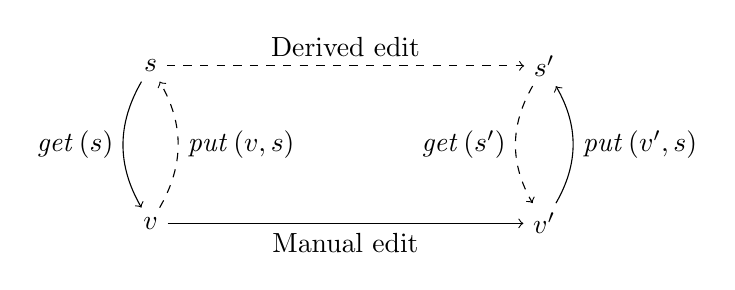
\begin{tikzpicture}
    \node[] (OS) at (0, 2) {$s$};
    \node[] (OV) at (0, 0) {$v$};
    \node[] (ES) at (5, 2) {$s'$};
    \node[] (EV) at (5, 0) {$v'$};
    
    \draw[dashed,->] (OS) -- (ES) node [midway, above] {Derived edit};
    \draw[->] (OV) -- (EV) node [midway, below] {Manual edit};
    \path[->] (OS) edge[bend left=-30] node[left] {$\mathit{get}\left(s\right)$} (OV);
    \path[dashed,->] (ES) edge[bend left=-30] node[left] {$\mathit{get}\left(s'\right)$} (EV);
    \path[dashed,->] (OV) edge[bend right=30] node[right] {$\mathit{put}\left(v, s\right)$} (OS);
    \path[->] (EV) edge[bend right=30] node[right] {$\mathit{put}\left(v', s\right)$} (ES); 
  \end{tikzpicture}
  \caption{Overview of a standard lens.}
  \label{fig:lens:overview}
\end{figure}

\section*{Current State of Research}
The most closely related work to ours is by St{\u{a}}nciulescu et al., which is
also a view-based editing method~\cite{stuanciulescu2016}. Their system is
defined in the formalisation of variational software called \emph{Choice Calculus}~\cite{walkingshaw2014}.
Choice calculus abstracts away the notation of \texttt{\#ifdef} statements into
a more formal syntax to simplify the definitions. A choice is then represented
using \(F \left<e_1, e_2\right>\), where $F$ is the presence condition of an
expression, $e_1$ is the expression that is executed when $F$ holds and $e_2$
the expression that is executed when $F$ does not hold. Our work will not be 
based on choice calculus, but rather on the conceptual structures of the Virtual
Platform.

In this previous work, the \emph{get} operator requires a \emph{choice}, with
which the programmer determines the set of variants included in the view (expressed
in terms of activated and deactivated features).
The \emph{put} operator requires another expression, called the \emph{ambition}.
The ambition is a way for the programmer to determine the set of variants to
which the changes should be applied. The way the \emph{put} operator deals with
this ambition, is by creating a new top-level choice (a representation of an
\texttt{\#ifdef}) in the form of \( \left(c \land a\right)\left<v', s\right> \).
Here, $c$ and $a$ are the chosen choice and ambition in the \emph{get} and
\emph{put} operators, $v'$ is the edited view and $s$ is the source from which
the view originated. This top-level choice is then minimised such that the
common parts are extracted from both branches.

The limitations of this work, as mentioned before, are twofold. The method
is not proven to be correct with the lens laws. The way the \emph{put}
operator works, does not allow changes to be propagated to a scope beyond
the \emph{choice} expression from the \emph{get} operator. This was a
deliberate design choice as it holds to the \emph{Edit Isolation Principle},
where changes can only be made to what is visible in the view. In this work,
we want to lift this restriction, as well as prove the lens laws.

\section{Running Example}\label{sec:background:example}
In this work, we will generally use the sample example system to show the workings of
the formalisations. This is a simple application that initially has three classes
embedded in one file. Our system has two features, namely an optional \emph{CLI} and
\emph{logging}. We have that \emph{logging} can only be enabled when \emph{CLI} is
enabled, guarded by a feature model. In the end, we want to be able for a developer
to work only on a part of the file, and then be able to also push these changes
back into the full source file.
